\subsection{Summary}
\label{subsec:resultssummary}

\begin{figure}[h!]
    \centering
    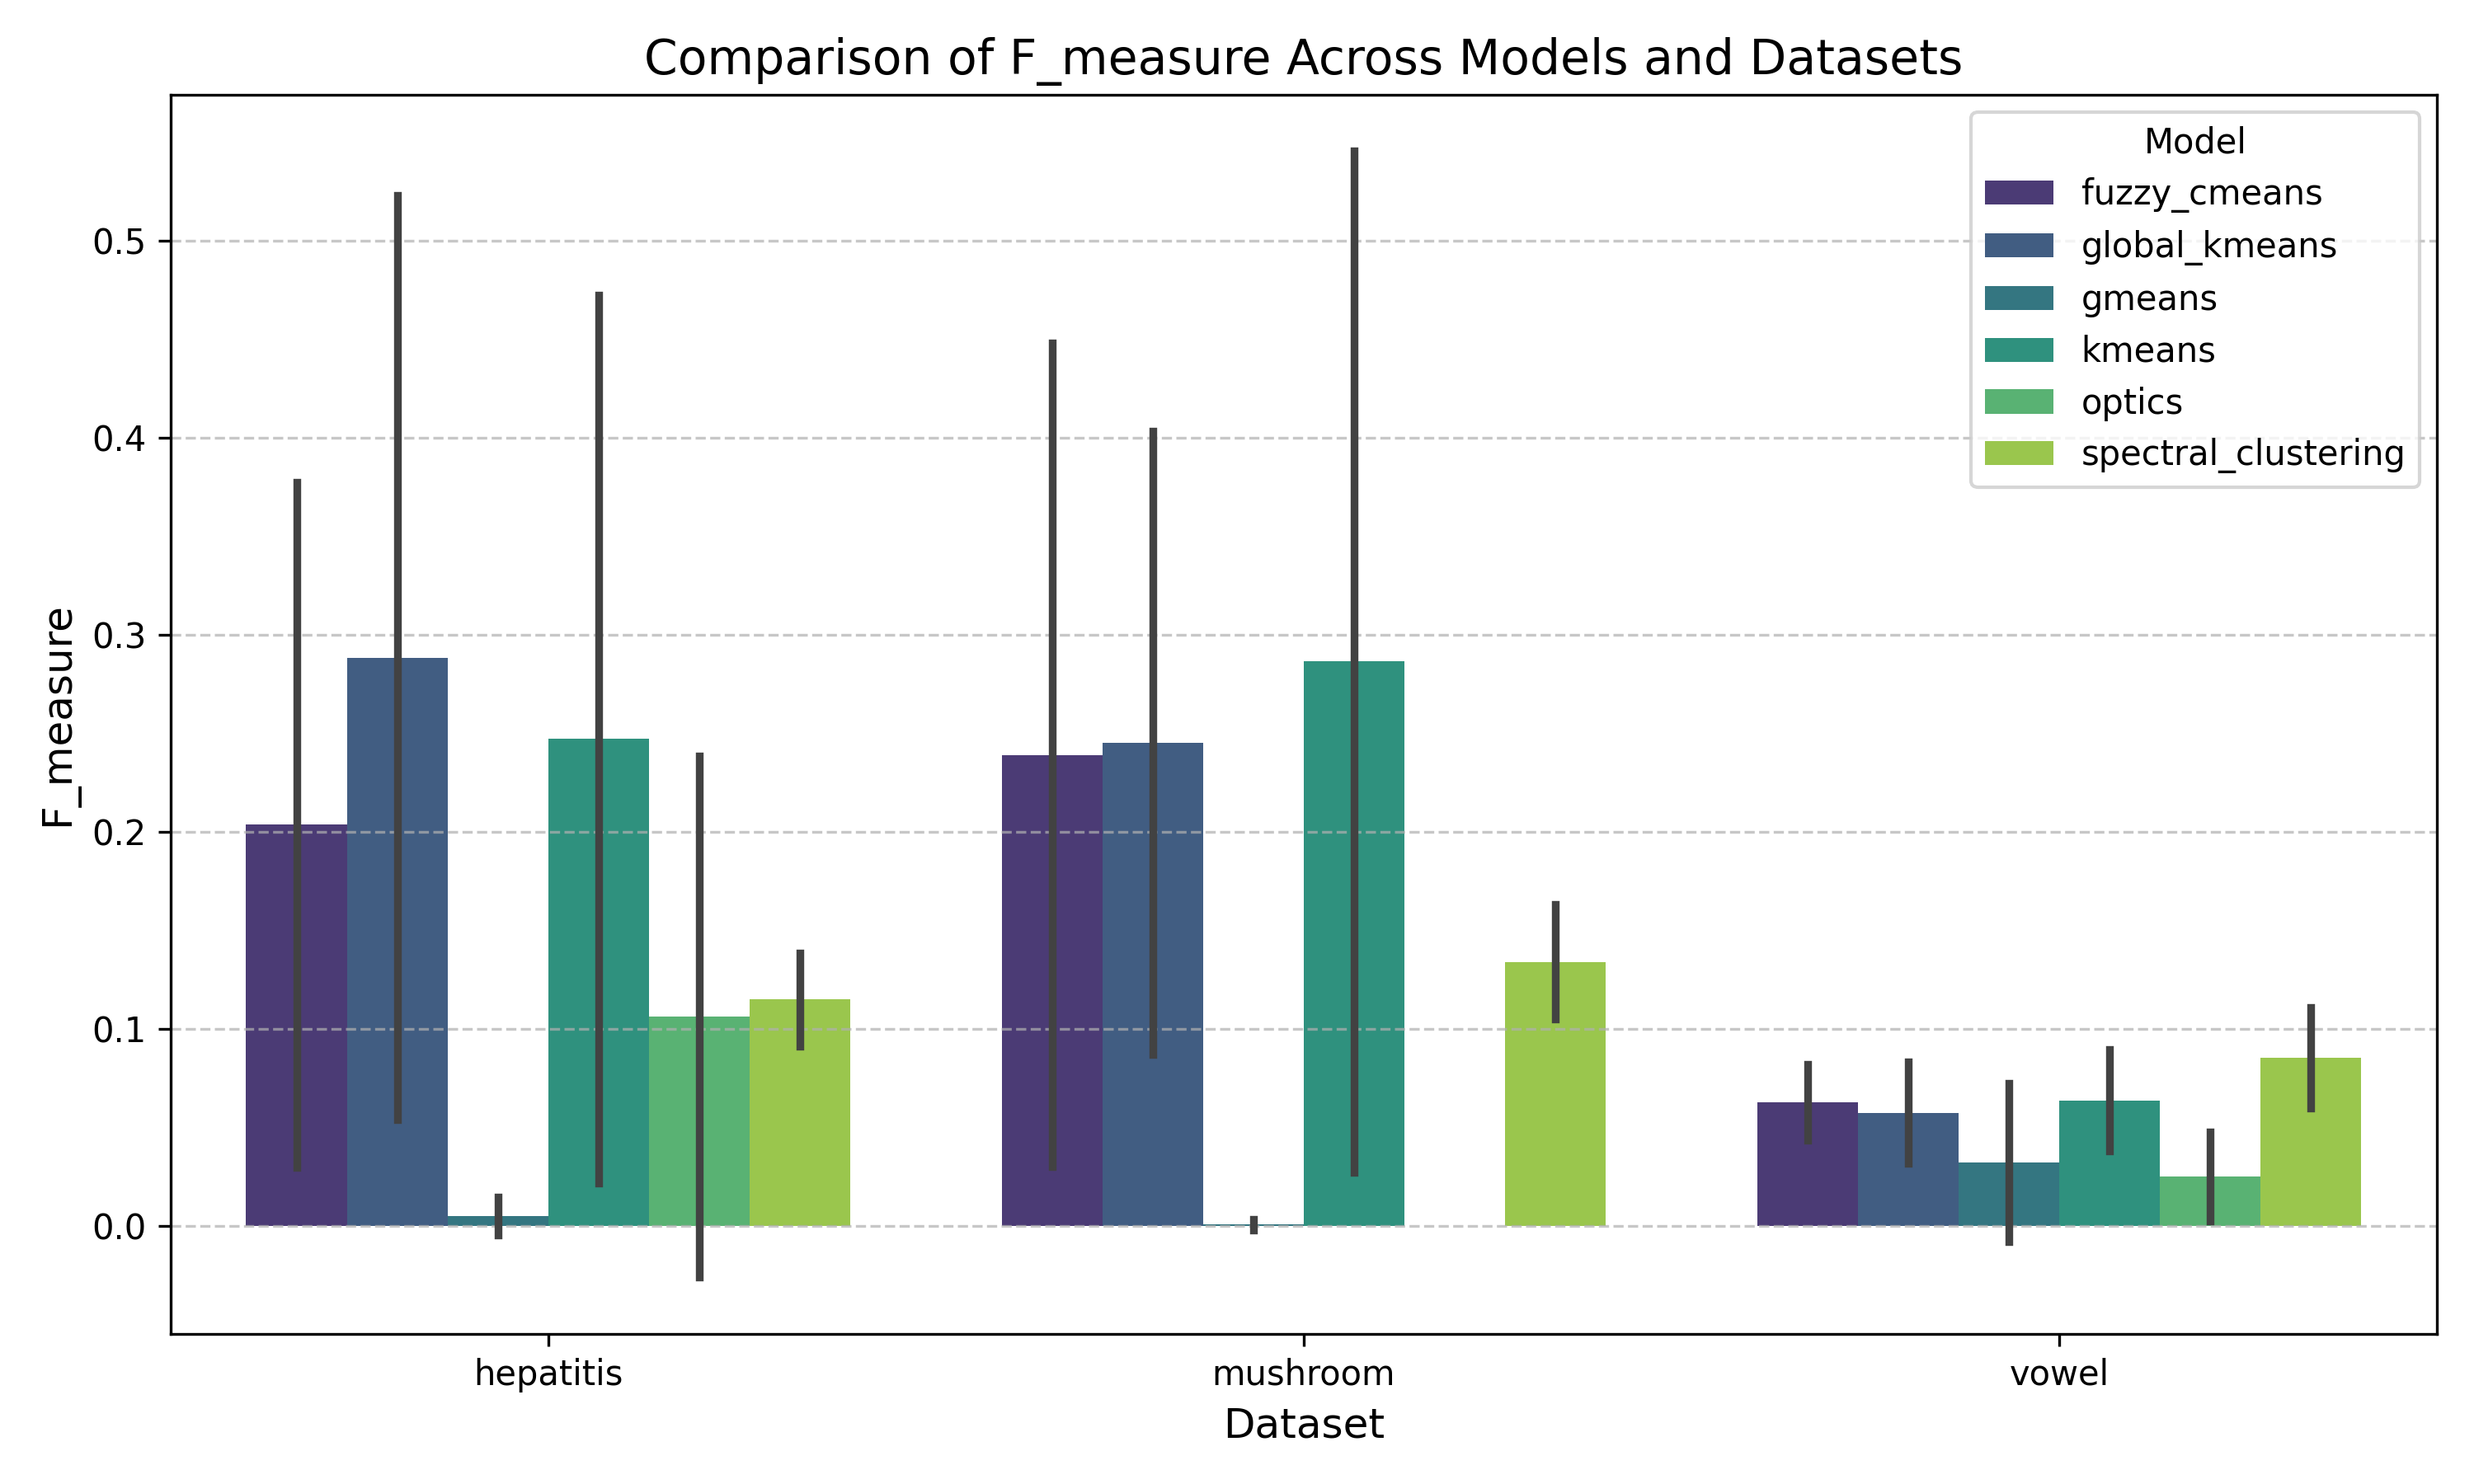
\includegraphics[width=0.5\textwidth]{figures/model_comparison_f_measure.png}
    \caption{F1 Score Comparison Across Datasets}
    \label{fig:model_comparison_f_measure}
\end{figure}

The Mushroom dataset, with its simple two-class structure, was best handled by K-Means,
Spectral Clustering, and Fuzzy C-Means. K-Means and Spectral Clustering achieved high F1 
scores when the cluster counts matched the natural class count. Fuzzy C-Means maintained
consistently high performance across a range of parameter combinations, while more complex 
methods like G-Means and OPTICS added no benefit.

The Hepatitis dataset, with moderate complexity and imbalanced classes, showed mixed results.
K-Means and Global K-Means performed well when clusters aligned with the natural classes. 
OPTICS and Fuzzy C-Means succeeded with careful tuning, with OPTICS favoring larger clusters and Fuzzy C-Means performing better with lower fuzziness values.
G-Means, however, exhibited instability due to sensitivity to hyperparameters like $max\_depth$ and strictness.

The Vowel dataset, characterized by high-class complexity and overlapping 
features, posed significant challenges. All algorithms struggled, with low F1 
scores across the board. Fuzzy C-Means showed some improvement with higher fuzziness 
values and larger cluster counts, but the gains were limited. Spectral Clustering 
and other methods failed to handle the dataset's complexity effectively, emphasizing the need for advanced clustering techniques.